\documentclass[letterpaper]{memoir}
% memoir commands to define the text block geometry
\setulmarginsandblock{1in}{*}{*}
\setlrmarginsandblock{1in}{*}{*}

\usepackage{xparse}
\usepackage{blindtext}
\usepackage{enumitem}
\usepackage{graphicx}

\usepackage{amsmath,mathtools,amssymb}
% See https://texblog.net/latex-archive/maths/amsmath-matrix/ 
% for an explanation of this extention of the amsmath matrix commands.
% It's a way to enable "augmented matrices" using a new optional argument:
%
% \begin{pmatrix}[cc|c]
%     1 & 2 & 3\\
%     4 & 5 & 9
%   \end{pmatrix}
%
\makeatletter
\renewcommand*\env@matrix[1][*\c@MaxMatrixCols c]{%
  \hskip -\arraycolsep
  \let\@ifnextchar\new@ifnextchar
  \array{#1}}
\makeatother

\usepackage{bm} % bold math package

\usepackage{booktabs}
\usepackage{multirow}
\usepackage{hyperref}
\usepackage{systeme}

\usepackage{tcolorbox}
    \tcbuselibrary{skins}
    \tcbuselibrary{raster}
    \tcbuselibrary{skins}
\usepackage{tikz}
    \usetikzlibrary{arrows.meta}
\usepackage{tkz-base}
\usepackage{tkz-fct}    
\usepackage{pgfplots}
    \pgfplotsset{compat=newest}

% for inserting blanks that the students fill in
\usepackage{dashundergaps} % for \gap
\dashundergapssetup{
    teacher-mode=false, % set to true to show answers 
    gap-format=underline,
    teacher-gap-format=underline,
    gap-font={\ECFAugie\MTversion{augie}\color{black}},
    gap-numbers=false,
    gap-widen=true,
    gap-extend-percent=100, % note: making this too big might create errors
    gap-number-format=\,\textsuperscript{\normalfont(\thegapnumber)},
}

\usepackage{emerald}
\usepackage[subdued]{mathastext}% no italic for Augie anyhow
    \MTDeclareVersion[n]{lmvtt}{T1}{lmvtt}{m}{n}
    \MTfamily{augie}
    \Mathastext[augie]

\newcommand{\myHeadFootStyle}{\footnotesize\sffamily}
\copypagestyle{myPagestyle}{empty}
%
% FIXME
% The following header definitions do NOT work right in all cases.
% I have found that the chapter title sometimes gets picked up from
% a chapter that begins on the NEXT PAGE. Not sure what's going on.
% So I abandoned embedding the info in the header and instead updated
% \myLesson to print it out, and that seems to work find.
%
% \makeoddhead{myPagestyle}
%     {\,}
%     {\,}
%     {\myHeadFootStyle\chaptername\,\thechapter\,\,\myCurrentChapterTitle}
% \makeevenhead{myPagestyle} 
%     {\,}
%     {\,}
%     {\myHeadFootStyle\chaptername\,\thechapter\,\,\myCurrentChapterTitle}
\makeoddfoot{myPagestyle}
    {\myHeadFootStyle\myCurrentBookTitle}
    {\myHeadFootStyle\thepage}
    {\myHeadFootStyle\thechapter.\themyLessonCounter\,\,\myCurrentLessonTitle}
\makeevenfoot{myPagestyle}
    {\myHeadFootStyle\thechapter.\themyLessonCounter\,\,\myCurrentLessonTitle}
    {\myHeadFootStyle\thepage}
    {\myHeadFootStyle\myCurrentBookTitle}


\begin{document}
\pagestyle{myPagestyle}
\checkandfixthelayout
\raggedbottom

\newcommand{\myEmph}{\bfseries\itshape}
\newcommand{\myClassName}{{\tagged{pre-AP}{pre-AP }}Algebra 2}

% So I can save/restore \fboxsep
\newlength{\mySavedFboxsep}
\newcommand{\mySaveFboxsep}{\setlength{\mySavedFboxsep}{\fboxsep}}
\newcommand{\mySaveAndSetFboxsep}[1]{
    \setlength{\mySavedFboxsep}{\fboxsep}
    \setlength{\fboxsep}{#1}
}
\newcommand{\myRestoreFboxsep}{\setlength{\fboxsep}{\mySavedFboxsep}}

% A centered tcolorbox
%
% #1 - options to pass to tcolorbox
%
\NewDocumentEnvironment{myCenteredBox}{m}{%
    \begin{center}
    \begin{tcolorbox}[#1]
}{
    \end{tcolorbox}
    \end{center}
}


% A centered system of equations
%
\NewDocumentCommand{\myCenteredSysteme}{m}{%
    \begin{center}\systeme{#1}\end{center}
}

%
% This specialized command is my way of typesetting a table for
% students to use when solving systems of equations using matrices.
%
% - I make it really wide, because I need horizontal space. The increase in margin width 
%   is adjustable, but frankly, there are a lot of hard-coded dimensions in the table, so
%   I'm not positive that generality works well.
%
% - I put the content in a tikz picture with an OPAQUE background, since I 
%   plan to overlay this on top of Examples, which have dotted boxes around 
%   them at the "normal" margins.
%
% - The table uses the multirow package so that I can have the "Solution" box span two cells.
%
\NewDocumentCommand{\myWideMatrixTable}{O{-0.7in}}{
    \begin{adjustwidth}{#1}{#1}
        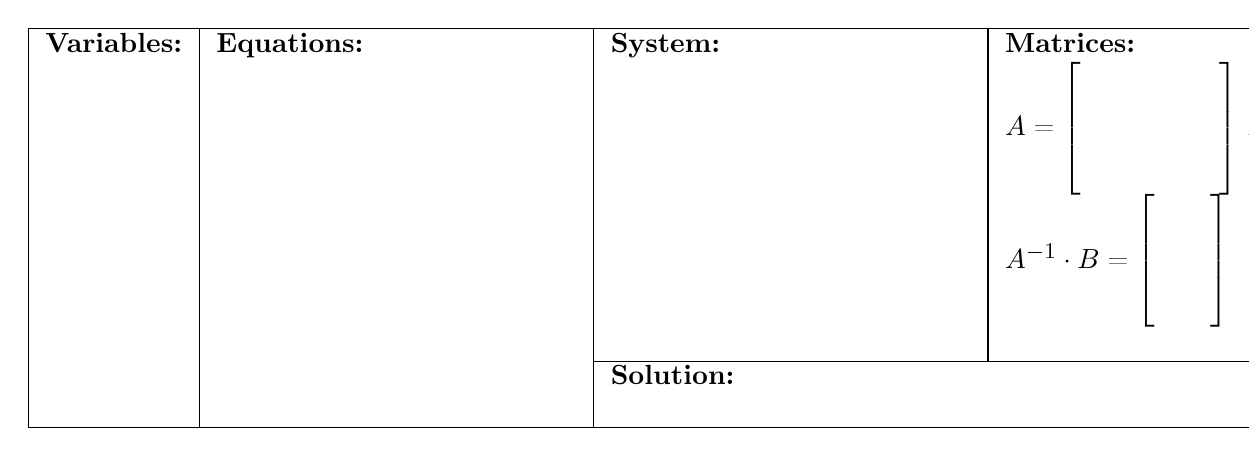
\begin{tikzpicture}
            \node
            [
                text width=1.25\textwidth, %I dinked with the multiplier to get balanced margins
                fill=white!30, 
                fill opacity=1,
                text opacity=1,
                inner sep=0pt,
            ]
            {%
                \begin{tabular}{|l|m{1.8in}|m{1.8in}|m{2.1in}|}
                    \hline
                    {\bfseries\scshape Variables:} & {\bfseries\scshape Equations:} & {\bfseries\scshape System:} & {\bfseries\scshape Matrices:} \\
                    % & & & \\
                    & & & 
                    \(
                        A = 
                        \begin{bmatrix}
                            \phantom{99} & \phantom{99} & \phantom{99} \\
                            \phantom{99} & \phantom{99} & \phantom{99} \\
                            \phantom{99} & \phantom{99} & \phantom{99} \\
                            \phantom{99} & \phantom{99} & \phantom{99} \\
                        \end{bmatrix}
                    \)
                    \(
                        B = 
                        \begin{bmatrix}
                            \phantom{999}\\
                            \phantom{999}\\
                            \phantom{999}\\
                            \phantom{999}\\
                    \end{bmatrix}
                    \)
                    \\
                    & & &
                    \(
                        A^{-1}\cdot B = 
                        \begin{bmatrix}
                            \phantom{9999}\\
                            \phantom{999}\\
                            \phantom{999}\\
                            \phantom{999}\\
                    \end{bmatrix}
                    \)
                    \\
                    & & & \\ \cline{3-4}
                    & & 
                    \multicolumn{2}{l|}{\bfseries\scshape Solution:}
                    \\ 
                    & & 
                    \multicolumn{2}{l|}{\,}
                    \\ 
                    \hline
                \end{tabular}
            };
        \end{tikzpicture}
    \end{adjustwidth}
}

%
% I am piggy-backing off of the standard memoir document
% divisions:
%
% book    -- is for the name of my class (eg, Alg2)
% part    -- is for the semester 
% chapter -- is for units
%
% To do this, I need to change the default value of various
% division-related commands. That's what the following is for.

%----- CLASS ---------
\newcommand{\myCurrentBookTitle}{}
\let\myOldBook\book
\renewcommand{\book}[1]{
    \renewcommand{\myCurrentBookTitle}{#1}
    \myOldBook{#1}
}
% I don't want roman numerals.
\makeatletter
\renewcommand*{\thebook}{\@arabic\c@book}
\makeatother
% I just want the title (not "Class 1 <title>")
\renewcommand{\printbookname}{}
\renewcommand{\booknamenum}{}
\renewcommand{\printbooknum}{}


%----- SEMESTER -------
% I don't want roman numerals.
\makeatletter
\renewcommand*{\thepart}{\@arabic\c@part}
\makeatother


%----- UNIT -----------
\renewcommand{\chaptername}{Unit}
\newcommand{\myCurrentChapterTitle}{}
\let\myOldChapter\chapter
\renewcommand{\chapter}[1]{
    \renewcommand{\myCurrentChapterTitle}{#1}
    \myOldChapter{#1}
}
%-------- LESSONS --------------

\newcounter{myLessonCounter}[chapter] 
\newcommand{\myCurrentLessonTitle}{}
\newcommand{\myFullLessonNumber}{}  % for example 2.3b

% #1 - lesson title
% #2 - optional lesson number (default increments from previous)
% #3 - optional lesson number suffix (eg, 'a' or 'b')
%
\NewDocumentCommand{\myLesson}{ m o O{} }{
    \cleartorecto
    \renewcommand{\myCurrentLessonTitle}{#1}
    \IfValueTF{#2}
        {\setcounter{myLessonCounter}{#2}}
        {\stepcounter{myLessonCounter}}
    \renewcommand{\myFullLessonNumber}{\thechapter.\themyLessonCounter#3}
    \noindent
    \begin{minipage}[b]{0.25\textwidth}
        {
            \HUGE\bfseries\sffamily\myFullLessonNumber
        }
    \end{minipage}
    \begin{minipage}[b]{0.74\textwidth}
        \begin{flushright}
            {\sffamily\chaptername\,\thechapter\,\,\myCurrentChapterTitle}\\
            \vspace{0.75\baselineskip}
            {\Huge\bfseries\sffamily#1}
        \end{flushright}
    \end{minipage}
    
    \noindent\rule{\textwidth}{1.25pt}
    \par
}

%-------- ANNOTATIONS (in boxes) --------------
%
% I use the term "annotations" to capture the common
% infrastructure I use to define Objectives, Vobabulary & Concepts.
%

% font and styling commands for
% Objectives, Voculary, Key Concepts, etc...
\newcommand{\myAnnotationStyling}{\bfseries\large}

% #1 : name of the kind of annotation (Objectives, ...)
% #2 : title text to go with the annotation
\NewDocumentEnvironment{myAnnotate}{ m m }{
    \begin{tcolorbox}[
        colbacktitle=blue!10!white,
        colback=white,
        coltitle=black,
        fonttitle={\myAnnotationStyling},
        title={#1: },
        after title={\normalfont\itshape#2},
        ]
}{
    \end{tcolorbox}
}

% #1 : name of the kind of annotation 
% #2 : title 
\NewDocumentEnvironment{myTabularAnnotate}{ m m }{
    \begin{myAnnotate}{#1}{#2}
    \begin{tabular}{r|l}
}{
    \end{tabular}
    \end{myAnnotate}
}
% #1 - column 1 text
% #2 - column 2 text
\NewDocumentCommand{\myRow}{mm}{{\bfseries\itshape \textcolor{blue}{#1}}&#2\\[1ex]}

% #1 : name of the kind of annotation 
% #2 : title 
% #3 : text before the list starts
\NewDocumentEnvironment{myListAnnotate}{ m m o }{
    \begin{myAnnotate}{#1}{#2}
    \IfValueT{#3}{#3}
    \begin{enumerate}[itemsep=0pt,]
}{
    \end{enumerate}
    \end{myAnnotate}
}
% #1 - column 1 text
% #2 - column 2 text
\NewDocumentCommand{\myItem}{mm}{\item{\bfseries\itshape \textcolor{blue}{#1}} #2}



%----------- OBJECTIVES , VOCABULARY, CONCEPTS ---------------
\newenvironment{myObjectives}{
    \begin{myListAnnotate}{Objectives}{}
}{
    \end{myListAnnotate}
}
\newcommand{\myObjective}[2]{
    \myItem{#1}{#2}
}

\newenvironment{myVocabulary}{
    \begin{myTabularAnnotate}{Vocabulary}{}
}{
    \end{myTabularAnnotate}
}
\newcommand{\myDefinition}[2]{
    \myRow{#1}{#2}
}

\NewDocumentEnvironment{myConcept}{m}{
    \begin{myAnnotate}{Key Concept}{#1}
}{
    \end{myAnnotate}
}

\NewDocumentEnvironment{myConceptSteps}{m}{
    \begin{myListAnnotate}{Key Concept}{#1}[Follow these steps.]
}{
    \end{myListAnnotate}
}
\newcommand{\myStep}[2]{
    \myItem{#1.}{#2}
}

%----------- EXAMPLEs ---------------
\newcounter{myExampleCounter}[myLessonCounter] 

% #1 A statement of the example problem.
% #2 borderline style (dashed, transparent, etc... )
%
\NewDocumentEnvironment{myExample}{sm}{%
    \vspace{1.25em}
    \IfBooleanTF{#1}%
    {
        \tcbset{
        borderline east={0.5pt}{0pt}{white,dashed},
        borderline west={0.5pt}{0pt}{white,dashed},
        }
    }
    {
        \tcbset{
        borderline east={0.5pt}{0pt}{black,dashed},
        borderline west={0.5pt}{0pt}{black,dashed},
        }
    }
    \begin{tcolorbox}[
        enhanced,
        sharp corners, 
        colback=white,
        boxrule=0pt,
        borderline north={0.5pt}{0pt}{black,dashed},
        borderline south={0.5pt}{0pt}{black,dashed},
        % borderline east={0.5pt}{0pt}{blue,thick},
        % borderline west={0.5pt}{0pt}{blue,thick},
        ]
        \stepcounter{myExampleCounter}
        {\myAnnotationStyling Example \themyExampleCounter:} {\large #2}
        \tcblower
}{
    \end{tcolorbox}
}

% #1 amount of vspace for the blank space
% #2 A statement of the example problem
\NewDocumentCommand{\myBlankExample}{mm}{
    \begin{myExample}{#2}
        \vspace{#1}
    \end{myExample}
}

% #1 optional horizontal width (defaults to text width)
% #2 required vertical height
% #3 text
%
% Note: This command does not increment the example counter.
%
\NewDocumentCommand{\myEmptyExampleBox}{ o m m}{
    \begin{center}
        \IfValueT{#1}{\tcbset{width=#1}} % for some reason, I am unable to conditionally insert in the properties list
        \begin{tcolorbox}[
            enhanced,
            sharp corners, 
            colback=white,
            boxrule=0pt,
            borderline={0.75pt}{0pt}{black,dotted},
            ]
            #3
            \vspace{#2}
        \end{tcolorbox}
    \end{center}
}

% Units are based on \chapter. But we're not doing chapters
% in this one-lesson file. So we "fake out" the relevant 
% chapter (unit) number and title.
\renewcommand{\thechapter}{1} 
\renewcommand{\myCurrentChapterTitle}{Introduction to Functions}

\myLesson{Attributes of Relations and Functions}[2]

\begin{myObjectives}
    \tagged{on-level}{
        \myObjective{solve}{one-step linear equations}
    }
    \myObjective{solve}{multi-step linear equations}
    \myObjective{solve}{formulas for one variable given the value of all the other variables}
    \myObjective{solve}{formulas for one variable in terms of the other variables}
\end{myObjectives}

\begin{myVocabulary}
    \myDefinition{equation}{algebraic expressions connected with an $=$ sign}
    \myDefinition{formula}{an equation with more than one variable}
    \myDefinition{inverse operation}{
        two operations that to \emph{opposite} things 
        (They \emph{undo} each other.)
    }
    \myDefinition{solve}{find the value of a variable that makes an equation true}
\end{myVocabulary}




\section{Factoring Cubic Polynomials by Grouping}


\begin{myCenteredBox}[width=4.75in,]
    Sometimes you can \gap{factor} cubic polynomials by \gap{grouping} 
    using this pattern.
    {\Large
    \begin{equation*}
        a(c+d) + b(c+d) = (a+b)(c+d)
    \end{equation*}
    }
\end{myCenteredBox}

\begin{myConceptSteps}{~to factor cubic polynomials by grouping \dots}
    \myStep{groups}{Group the first two terms together and the last two terms together.}
    \myStep{GCFs}{Factor out GCFs from each group.}
    \myStep{rewrite}{Write the result as two factored polynomials.}
\end{myConceptSteps}


\begin{taggedblock}{on-level}
    \begin{my2Problems}[\large]{3.5in}[
        Factor these cubic polynomials. Hint: Always remove a GCF first (if you can).
        ]
        {
            $ 4x^3 + x^2 + 12x + 3 $
        }
        {
            $ 9x^3 - 12x^2 - 27x + 36 $
        }
    \end{my2Problems}
    \begin{myProblem}[\large]{3.5in}
        {
            $ 2r^3 - r^2 - 8r + 4 $
        }
    \end{myProblem}
\end{taggedblock}

\begin{taggedblock}{pre-AP}
    \begin{my2Problems}[\large]{3.5in}[
        Factor these cubic polynomials. Hint: Always remove a GCF first (if you can).
        ]
        {
            $ 35x^3 + 49x^2 + 25x + 35 $
        }
        {
            $ 6p^4 -8p^3 -24p^2 +32p $
        }
    \end{my2Problems}
\end{taggedblock}

\begin{my2Problems}[\normalsize]{1in}[%
    Here are equations for a transformed square root function.
    For each problem,
    \vspace{-1em}
    \begin{itemize}[nosep]
        \item Find the value of $a$ or $h$ or $k$. (You decide which one!)
        \item Describe (in words) the transformation from the parent function, $f(x)=\myRoot{x}$.
    \end{itemize}
    ]
    {
        $g(x) = 5 \myRoot{x}$
    }
    {
        $g(x) = \myRoot{x} + 3$
    }
\end{my2Problems}
\begin{my2Problems}[\normalsize]{1in}
    {
        $g(x) = \myRoot{x-7}$
    }
    {
        $g(x) = \frac{1}{3}\myRoot{x}$
    }
\end{my2Problems}



\begin{my2Problems}[\normalsize]{1in}[%
    Here are descriptions of transformations of the square root parent function.
    For each problem, write the corresponding equation of $g(x)$.
    ]
    {
        shift down by 8
    }
    {
        reflect across the $x$-axis
    }
\end{my2Problems}
\begin{my2Problems}[\normalsize]{1in}
    {
        stretch vertically be a factor of 2
    }
    {
        shift left by 6
    }
\end{my2Problems}





\section*{Finding the maximum,  minimum, domain, and range}

\begin{myConceptSteps}{
    To find the maximum and minimum of a quadratic function in standard form\dots
    }
    \myStep{$\mathbf a$}{
        Find $\mathbf a$ from the standard form equation.
    }
    \myStep{positive $a$}{
        The parabola {\bfseries\itshape opens up} if $a$ is positive.
        In that case, the vertex is a {\bfseries\itshape minimum},
        and there is no maximum.
    }
    \myStep{negative $a$}{
        The parabola {\bfseries\itshape opens down} if $a$ is negative.
        In that case, there is no minimum, and 
        the vertex is a {\bfseries\itshape maximum}.
    }
\end{myConceptSteps}

\myBlankExample{2.5in}{
    Find the maximum and minimum of this quadratic function:
    $y = 2x^2 + 4x - 3$
}

\myBlankExample{2.5in}{
    Find the maximum and minimum of this quadratic function:
    $y = -2x^2 - 4x + 3$
}


\begin{myConceptSteps}{
    To find the domain and range of a quadratic function in standard form\dots
    }
    \myStep{domain}{
        The domain of any quadratic function is {\bfseries\itshape all real numbers}.
    }
    \myStep{vertex}{
        Find coordinates of the vertex, $(x_V, y_V)$.
    }
    \myStep{positive $a$}{
        The parabola {\bfseries\itshape opens up} if $a$ is positive.
        In that case, the vertex is a {\bfseries\itshape minimum},
        and so the range is $y \geq y_V$.
    }
    \myStep{negative $a$}{
        The parabola {\bfseries\itshape opens down} if $a$ is negative.
        In that case, the vertex is a {\bfseries\itshape maximum},
        and so the range is $y \leq y_V$.
    }
\end{myConceptSteps}

\myBlankExample{2.5in}{
    Find the domain and range of this quadratic function:
    $y = 2x^2 + 4x - 3$
}

\myBlankExample{2.5in}{
    Find the domain and range of this quadratic function:
    $y = -2x^2 - 4x + 3$
}


\end{document}